\section{GraphBLAS Operations}
\label{Sec:Operations}

\tim{I found the previous version of this table to be hopelessly confusing.  Please check out my proposed replacement}
\scott{I support Tim's approach.  It basically removes everything that a descriptor could add.  I made some changes to notation to use angle brackets around the mask. How complete should this table be? I added entries that the GABB17 paper had but not the contents of the caption.}

The GraphBLAS operations are defined in the GraphBLAS math spec and summarized in 
Table~\ref{Tab:GraphBLASOps}.   In addition to methods that implement these
fundamental GraphBLAS operations, we support a number of variants that have been 
found to be especially useful in algorithm development.


%A mathematical overview of the the fundamental GraphBLAS operations that are
%discussed in this section are shown in Table~\ref{Tab:GraphBLASOps}.  This
%section also specifies variants to some of these operations where they have
%been found especially useful in algorithm development.
%


\comment{
\begin{table*}[h]
\hrule
\begin{center}
\caption{A Mathematical overview of the fundamental GraphBLAS operations supported.}
\label{Tab:GraphBLASOps}
\begin{tabular}{l|rrl}
{\sf Operation Name} & \multicolumn{3}{c}{Mathematical Description}  \\
\hline
{\sf mxm}          & $\matrix{C}([\neg]\matrix{M})$ & $[\oplus]=$ & $\matrix{A}^{[T]} \oplus.\otimes \matrix{B}^{[T]}$  \\
{\sf mxv}          & $\vector{u}(\left[\neg\right]\vector{m})$ & $\left[\oplus\right]=$ & $\matrix{A}^{\left[T\right]} \oplus.\otimes \vector{v}$  \\
{\sf vxm}          & $\vector{u}(\left[\neg\right]\vector{m})$ & $\left[\oplus\right]=$ & $\vector{v} \oplus.\otimes \matrix{A}^{\left[T\right]}$  \\
{\sf eWiseMult}    & $\matrix{C}(\left[\neg\right]\matrix{M})$ & $\left[\oplus\right]=$ & $\matrix{A}^{\left[T\right]} \otimes \matrix{B}^{\left[T\right]}$  \\
{\sf eWiseAdd}     & $\matrix{C}(\left[\neg\right]\matrix{M})$ & $\left[\oplus\right]=$ & $\matrix{A}^{\left[T\right]} \oplus  \matrix{B}^{\left[T\right]}$  \\
{\sf reduce} (row) & $\vector{u}(\left[\neg\right]\vector{m})$ & $\left[\oplus\right]=$ & $\oplus_j\matrix{A}^{\left[T\right]}(:,j)$  \\
{\sf apply}        & $\matrix{C}(\left[\neg\right]\matrix{M})$ & $\left[\oplus\right]=$ & $f(\matrix{A}^{\left[T\right]})$ \\
{\sf transpose}    & $\matrix{C}(\left[\neg\right]\matrix{M})$ & $\left[\oplus\right]=$ & $\matrix{A}^{\left[T\right]}$ \\
{\sf extract}      & $\matrix{C}(\left[\neg\right]\matrix{M})$ & $\left[\oplus\right]=$ & $\matrix{A}^{\left[T\right]}(\vector{i},\vector{j})$ \\
{\sf assign}       & $\matrix{C}(\left[\neg\right]\matrix{M})(\vector{i},\vector{j})$ & $\left[\oplus\right]=$ & $\matrix{A}^{\left[T\right]}$ \\
{\sf buildMatrix}  & $\matrix{C}(\left[\neg\right]\matrix{M})$ & $\left[\oplus\right]=$ & $\mathbb{S}^{m\times n}(\vector{i},\vector{j},\vector{v},\oplus_{dup})$ \\
{\sf buildVector}  & $\vector{u}(\left[\neg\right]\vector{m})$ & $\left[\oplus\right]=$ & $\mathbb{S}^{n}(\vector{i},\vector{v})$ \\
{\sf extractTuples}& $(\vector{i},\vector{j},\vector{v})$ & $=$ & $\matrix{A}(\left[\neg\right]\matrix{M})$ \\
\end{tabular}
\end{center}
\hrule
\end{table*}
}

\begin{table}[tb]
\hrule
\begin{center}
\caption{A Mathematical overview of the fundamental GraphBLAS operations supported
in this specification.  Input matrices $\matrix{A}$ and $\matrix{B}$ may be 
optionally transposed. Use of an optional accumulate with existing values in the output object is indicated. Use of an optional mask is indicated, for example when applied to the output matrix, $\matrix{C}$, as 
$\matrix{C}\langle\matrix{M}\rangle$. The mask or its structural complement 
controls which values are written into the output object.  An additional option
not shown here, is whether the all values in the output object are replaced or only the values/locations that are being written (merge mode).}
\label{Tab:GraphBLASOps}
\newcommand{\odotsp}{\hspace{-0.2cm}\odot\hspace{-0.18cm}}
\begin{tabular}{l|rcrcl}
{\sf Operation Name} & \multicolumn{5}{c}{Mathematical Description}  \\
\hline
{\sf mxm}          & $\matrix{C}\langle\matrix{M}\rangle$ & $=$ & $\matrix{C}$ & $\odotsp$ & $\matrix{A} \oplus.\otimes \matrix{B}$  \\
{\sf mxv}          & $\vector{w}\langle\vector{m}\rangle$ & $=$ & $\vector{w}$ & $\odotsp$ & $\matrix{A} \oplus.\otimes \vector{u}$  \\
{\sf vxm}          & $\vector{w}^T\langle\vector{m}^T\rangle$ & $=$ & \hspace{-0.18cm}$\vector{w}^T$ & $\odotsp$ & $\vector{u}^T \oplus.\otimes \matrix{A}$  \\
{\sf eWiseMult}    & $\matrix{C}\langle\matrix{M}\rangle$ & $=$ & $\matrix{C}$ & $\odotsp$ & $\matrix{A} \otimes \matrix{B}$  \\
                   & $\vector{w}\langle\matrix{m}\rangle$ & $=$ & $\vector{w}$ & $\odotsp$ & $\vector{u} \otimes \vector{v}$  \\
{\sf eWiseAdd}     & $\matrix{C}\langle\matrix{M}\rangle$ & $=$ & $\matrix{C}$ & $\odotsp$ & $\matrix{A} \oplus  \matrix{B}$  \\
                   & $\vector{w}\langle\matrix{m}\rangle$ & $=$ & $\vector{w}$ & $\odotsp$ & $\vector{u} \oplus \vector{v}$  \\
{\sf reduce} (row) & $\vector{w}\langle\vector{m}\rangle$ & $=$ & $\vector{w}$ & $\odotsp$ & $\left[\oplus_j\matrix{A}(:,j)\right]$  \\
{\sf reduce} (scalar) & $s$ & $=$ & $s$ & $\odotsp$ & $\left[\oplus_{i,j}\matrix{A}(i,j) \right]$  \\
                      & $s$ & $=$ & $s$ & $\odotsp$ & $\left[\oplus_i\matrix{u}(i) \right]$  \\
{\sf apply}        & $\matrix{C}\langle\matrix{M}\rangle$ & $=$ & $\matrix{C}$ & $\odotsp$ & $f_u(\matrix{A})$ \\
                   & $\vector{w}\langle\matrix{m}\rangle$ & $=$ & $\vector{w}$ & $\odotsp$ & $f_u(\vector{u} )$  \\
{\sf transpose}    & $\matrix{C}\langle\matrix{M}\rangle$ & $=$ & $\matrix{C}$ & $\odotsp$ & $\matrix{A}^T$ \\
{\sf extract}      & $\matrix{C}\langle\matrix{M}\rangle$ & $=$ & $\matrix{C}$ & $\odotsp$ & $\matrix{A}(\array{i},\array{j})$ \\
                   & $\vector{w}\langle\matrix{m}\rangle$ & $=$ & $\vector{w}$ & $\odotsp$ & $\vector{u}(\array{i})$ \\
%{\sf extract} (column) & $\matrix{w}\langle\vector{m}\rangle$ & $=$ & $\matrix{w}$ & $\odotsp$ & $\matrix{A}(\array{i}, j)$ \\
{\sf assign}       & $\matrix{C}\langle\matrix{M}\rangle(\array{i},\array{j})$ & $=$ & $\matrix{C}$ & $\odotsp$ & $\matrix{A}$ \\
                   & $\vector{w}\langle\vector{m}\rangle(\array{i})$ & $=$ & $\vector{w}$ & $\odotsp$ & $\matrix{u}$ \\
%& & & \\
%& \multicolumn{3}{c}{Input/Output Operations} \\
%{\sf Matrix\_build}  & $\matrix{C}$ & $=$ & $\mathbb{S}^{m\times n}(\array{i},\array{j},\array{v},\oplus_{dup})$ \\
%{\sf Vector\_build}  & $\vector{w}$ & $=$ & $\mathbb{S}^{n}(\array{i},\array{v},\oplus_{dup})$ \\
%{\sf Matrix\_extractTuples} & $(\array{i},\array{j},\array{v})$ & $=$ & $\matrix{A}$ \\
%{\sf Vector\_extractTuples} & $(\array{i},\array{v})$ & $=$ & $\matrix{u}$ \\
\end{tabular}
\end{center}
\hrule
\end{table}

\paragraph{Domains and Casting}

A GraphBLAS operation is only valid when the domains of the GraphBLAS objects are
mathematically consistent.  The C programming language defines implicit casts 
between ``plain old'' data types.  For example, floats, doubles and ints can be 
freely mixed according to the rules defined for implicit casts.  It is the 
responsibility of the user to assure that these casts are appropriate for the 
algorithm in question.  For example, a cast to int implies truncation of a floating 
point type.  Depending on the operation, this truncation error could lead to
erroneous results.  Furthermore, casting a wider type onto a narrower type can lead 
to overflow errors.  The GraphBLAS operations do not attempt to protect a user from 
these sorts of errors.

When user-define types are involved, however, GraphBLAS requires strict equivalence
between types and no casting is supported.  If GraphBLAS detects these mismatches,
it will return a domain mismatch error conditions.

\begin{figure}
    \hrule
    \begin{center}
        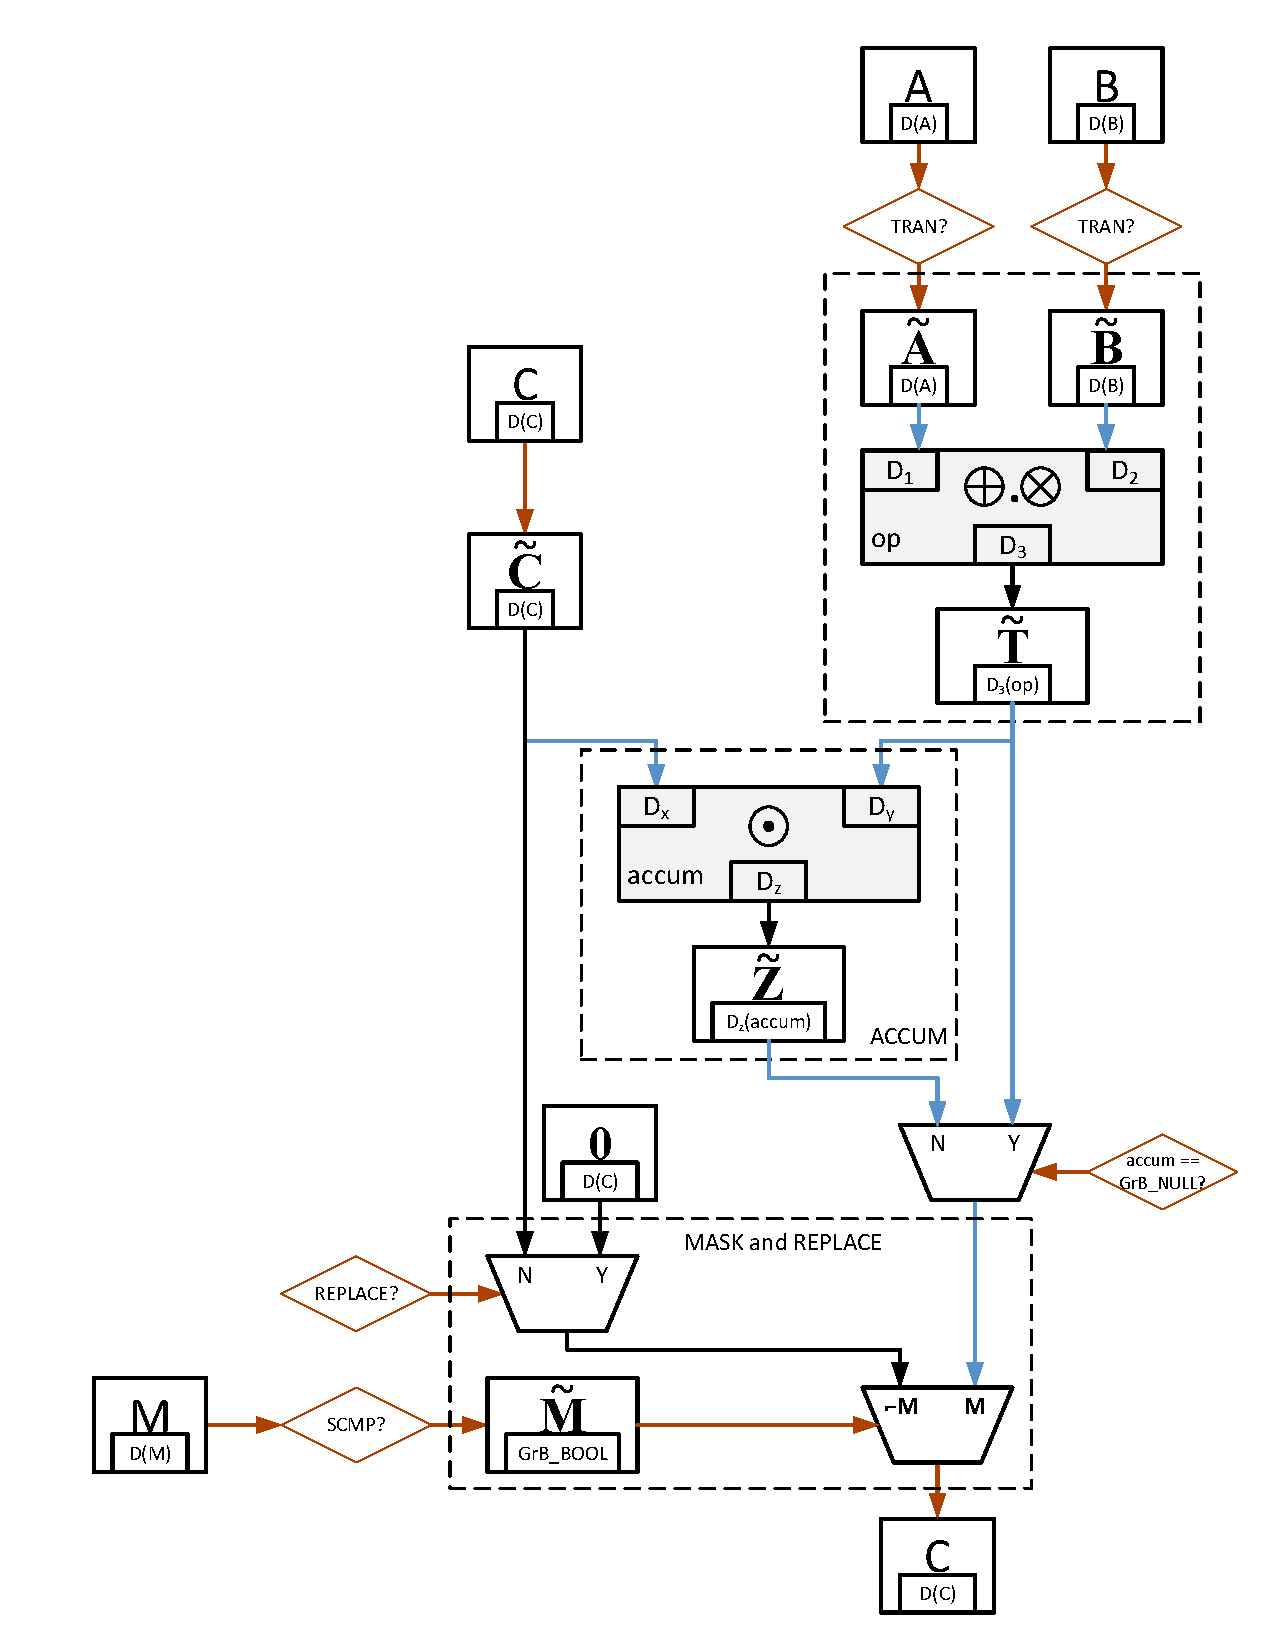
\includegraphics[width=5.5in]{mxm_operation_flowchart.pdf}
    \end{center}
    \caption{Flowchart for the GraphBLAS operations. Although shown specifically for
	the mxm operation, many elements are common to all operations: such as the ``{\sf ACCUM}'' 
	and ``{\sf MASK and REPLACE}'' blocks.  Orange arrows denote where ``as if copy''
    takes place (including both collections and descriptor settings).  Blue arrows
    indicate where casting may occur between different domains.}
    \label{Fig:mxmFlowchart}
    \hrule
\end{figure}

\paragraph{Dimensions and Transposes}

GraphBLAS operations also make assumptions about the numbers of dimensions and 
sizes of vectors and matrices in an operation.   An operation will test these 
sizes and report an error if they are not \emph{shape compatible}.  For example, when multiplying 
two matrices, $\matrix{C} = \matrix{A} \times \matrix{B}$, the number of rows of 
$\matrix{C}$ must equal the number of rows of $\matrix{A}$, the number of columns 
of $\matrix{A}$ must match the number of rows of $\matrix{B}$, and the number of 
columns of $\matrix{C}$ must match then number of columns of $\matrix{B}$.  This 
is the behavior expected given the mathematical definition of the operations.   

For most of the GraphBLAS operations involving matrices, an optional descriptor 
can modify the matrix associated with an input GraphBLAS matrix object.  For 
example, if an input matrix is an argument to a GraphBLAS operation and the 
associated descriptor indicates the transpose option, then the operation occurs 
as if on the transposed matrix.  In this case, the relationships between the 
sizes in each dimension shift in the mathematically expected way. 

\paragraph{Masks and Structural Complements}

%
% Note ... I've written this assuming the treatment of mask that Aydin and Tim
% prefer.  We'll change this text is we go the way Jose wants us to go.
%

When a GraphBLAS operation supports the use of an optional mask, that mask is
specified through a GraphBLAS vector (for one-dimensional masks) or
a GraphBLAS matrix (for two-dimensional masks).  When a mask is used, it is 
applied to the result from the operation whereever the mask evaluates to true, 
and then that result is either assigned 
to the provided output matrix/vector or, if a binary accumulation operation is 
provided, the result is accumulated into the corresponding elements of the provided 
output matrix/vector.

Given a GraphBLAS vector $\vector{v} = \langle D,N, \{ (i,v_i) \} \rangle$, a
one-dimensional mask $\vector{m} = \langle N, \{ i : \mbox{\tt (bool)}v_i = \true \} \rangle$
is derived for use in the operation, where $\mbox{\tt (bool)}v_i$ denotes
casting the value $v_i$ to a Boolean value (\true\ or \false).
We note that, if cast is disallowed for the mask by the operation descriptor, then
$\bold{D}(\vector{v})$ must be {\sf GrB\_BOOL}.

Given a GraphBLAS matrix $\matrix{A} = \langle D, M, N, \{ (i,j,A_{ij}) \} \rangle$,
a two-dimensional mask $\matrix{M} = \langle M,N, \{ (i,j) : \mbox{\tt (bool)}A_{ij} = \true \} \rangle$
is derived for use in the operation, where $\mbox{\tt (bool)}A_{ij}$ denotes
casting the value $A_{ij}$ to a Boolean value (\true\ or \false).

In both the one- and two-dimensional cases, the mask may go through a structural
complement operation ($\S$~\ref{Sec:Masks}) as specified in the descriptor, before 
a final mask is generated for use in the operation.

When the descriptor of an operation with a mask has specified that 
the {\sf GrB\_REPLACE} value is to be applied to the output ({\sf GrB\_OUTP}),
then anywhere the mask is false (i.e., unmasked), the corresponding location in
the output should be cleared.

\scott{We need a more explicit discussion/specification regarding
masks and accumulation and their interaction (perhaps the diagram Manoj
projected at the SC15 BoF.} \jose{Agree. Need to find the proper place
for it.}

\paragraph{Compliance}

We follow a \emph{prescriptive} approach to the definition of the semantics
of GraphBLAS operations. That is, for each operation we give a recipe for
producing its outcome.
It should be understood that any implementation that produces the same outcome,
and follows the GraphBLAS execution model (\S~\ref{Sec:ExecutionModel}) and
error model (\S~\ref{Sec:ErrorModel}), is a conforming implementation.
